%&presentatie
%% !TeX program = pdflatex

\def\rootpath{../../..}

\makeatletter
    \edef\input@path{{\rootpath}}
\makeatother

\documentclass{cursuspresentatie}

%\newif\ifishandout
\ishandoutfalse
%\ishandouttrue

\ifishandout
\documentclass[handout,aspectratio=32]{beamer}
\else
\documentclass[aspectratio=32]{beamer}
\fi

\usepackage[tabsize=4]{highlightlatex}

\setbeamertemplate{caption}[numbered]

\usecolortheme{rose}
%\useinnertheme[shadow]{rounded}
\useinnertheme{rounded}

\usetheme{Dresden}
\usecolortheme{dolphin}
\useoutertheme{miniframes}

\usepackage{subfiles}
\usepackage{amsmath,amssymb,amsthm,commath,mathtools}
\usepackage{esint}
\usepackage{enumerate}
\usepackage{subcaption}
\usepackage{graphicx}
\usepackage{xcolor}
\usepackage{adjustbox}
\usepackage{soul}
\usepackage{booktabs}
\usepackage{tabularx}
\usepackage{environ}
\usepackage[dutch]{babel}
\usepackage[utf8]{inputenc}
\usepackage{fancyvrb}
\usepackage{marvosym}
\usepackage{csquotes}
\usepackage[style=numeric]{biblatex}
\usepackage{textcomp}
%\usepackage{enumitem}
\usepackage{hyperref}
\usepackage{xkeyval}

\addbibresource{\subfix{assets/fakebib.bib}}

\DeclareMathOperator{\Image}{Image}

% Source: https://tex.stackexchange.com/questions/41683/why-is-it-that-coloring-in-soul-in-beamer-is-not-visible
\let\UL\ul
\makeatletter
\renewcommand\ul{
	\let\set@color\beamerorig@set@color
	\let\reset@color\beamerorig@reset@color
	\UL
}

\let\ST\st
\makeatletter
\def\st#1{
	\begingroup
	\let\set@color\beamerorig@set@color
	\let\reset@color\beamerorig@reset@color
	\def\SOUL@uleverysyllable{%
		\rlap{%
			%\color{red}
			\the\SOUL@syllable
			\SOUL@setkern\SOUL@charkern}%
		\SOUL@ulunderline{%
			\phantom{\the\SOUL@syllable}}%
	}%
	\ST{#1}%
	\endgroup
}
\makeatother
% https://tex.stackexchange.com/questions/71051/strikeout-in-different-color-appears-behind-letters-not-on-top-of-them

\setulcolor{red}
\setstcolor{red}

% Override if you want. Else you can delete it.
%\colorlet{curlyBrackets}{red!50!blue}
%\colorlet{squareBrackets}{blue!50!white}
%\colorlet{codeBackground}{gray!10!white}
%\colorlet{comment}{green!40!black}

\updatehighlight{
	name = default,
	color = {blue!90!black},
	add = {
		\knowncommand, \figref, \textcolor, \maketitle, \subsubsection,
		\textasciigrave, \textasciiacute, \tag, \middle, \mathbb, \abs,
		\mathcal, \middle, \dfrac, \subfile, \autoref, \eqref, \cites,
		\tableofcontents, \printbibliography, \fullcite, \parencite,
		\addbibresource, \DeclareLanguageMapping, \textcite, \intertext,
		\sum, \dif, \norm, \text, \dod, \dpd, \int, \partial,
		\DeclareMathOperator
	},
	name = structure,
	add = {
	},
}

\updatehighlight{
	name = greenDollar,
	style = {\itshape\color{green!70!black}},
	add = {
		% The dollar sign is provided an extra time just to
		% calm down TeXstudio's code highlighting.
		$, $
	},
	name = accentA,
	color = green!60!black,
	add = {
		\inAccA
	},
	%
	name = accentB,
	color = red!60!black,
	add = {
		\inAccB, \includegraphics
	},
	%
	name = accentC,
	color = orange!100!black,
	add = {
		\inAccC
	}
}

\lstset{tabsize=4}
\def\defaultgobble{8}

%\hllconfigure{
%	gobbletabs=3,
%}

\def\Zphantomconceal#1#2{%
	\only<#2->{\rlap{#1}}\phantom{#1}%
	%\only<#2->{#3}\unless\ifishandout\only<-#1>{\phantom{#3}}\fi
}

\def\phantomconceal#1#2{%
	\Zphantomconceal{#1}{#2}%
}

\newcommand\hideformula[2][2]{%
	%\hll|$| \only<2->{\hll|\\sqrt\{2\}|}\only<-1>{??} \hll|$|
	\hll|$| \phantomconceal{\hll|#2|}{#1} \hll|$|
}

\newcommand\hidelatex[2][2]{%
	\phantomconceal{\hll|#2|}{#1}
}%

\newcount\showcount

%\newcommand\showformula[2]{%
%	#1 & %
%	\expandafter\hideformula\expandafter[\the\showcount]{#2}%
%}
%
%\newcommand\showformula[2]{%
%	\global\showcount=\numexpr\showcount + 1\relax
%	\showformula*{#1}{#2}%
%}

\makeatletter

\def\showformula@i#1#2{%
	#1 & %
	\expandafter\hideformula\expandafter[\the\showcount]{#2}%
}

%\def\showformula{%
%	\@ifstar{%
%		\global\showcount=\numexpr\showcount + 1\relax
%		\showformula@i
%	}{%
%		\showformula@i
%	}%
%}

\def\showformula#1#2{
	#1 & \global\showcount=\numexpr\showcount + 1\relax
	\expandafter\hideformula\expandafter[\the\showcount]{#2}%
}

\def\showformulaa#1#2{
	#1 & %
	\expandafter\hideformula\expandafter[\the\showcount]{#2}%
}

\def\showlatex#1#2{
	#1 & \global\showcount=\numexpr\showcount + 1\relax
	\expandafter\hidelatex\expandafter[\the\showcount]{#2}%
}

\def\showlatexx#1#2{
	#1 & %
	\expandafter\hidelatex\expandafter[\the\showcount]{#2}%
}

\makeatother

\newlength{\naturalwidth}
\newlength{\minimumwidth}
\newbox\naturalsizebox
\newcommand{\atleastwidth}[2][2cm]{%
	\savebox\naturalsizebox{#2}%
	\settowidth\naturalwidth{#2}%
	\naturalwidth=\wd\naturalsizebox
	\minimumwidth=\dimexpr #1\relax
	\leavevmode%(\the\naturalwidth, \the\minimumwidth)%
	\ifdim\naturalwidth<\minimumwidth\relax
	\makebox[\minimumwidth][l]{\usebox{\naturalsizebox}}%
	\else
	\usebox{\naturalsizebox}%
	\fi
}

\newcommand{\atleastwidthr}[2][2cm]{%
	\savebox\naturalsizebox{#2}%
	\settowidth\naturalwidth{#2}%
	\naturalwidth=\wd\naturalsizebox
	\minimumwidth=\dimexpr #1\relax
	\leavevmode%(\the\naturalwidth, \the\minimumwidth)%
	\ifdim\naturalwidth<\minimumwidth\relax
	\makebox[\minimumwidth][r]{\usebox{\naturalsizebox}}%
	\else
	\usebox{\naturalsizebox}%
	\fi
}

\lstset{framexleftmargin=0.25em,xleftmargin=0.25em}

\NewEnviron{bluebox}{
	\begingroup
		\adjustbox{cfbox=blue!40!white 2pt 10pt,valign=t,bgcolor=blue!5!white}{%
			\begin{minipage}[t]{\dimexpr\linewidth-24pt\relax}
				\BODY
			\end{minipage}%
		}%
	\endgroup
}

\newcounter{maxrecentdisplay}
\setcounter{maxrecentdisplay}{27}

\newcounter{recentcount}
\setcounter{recentcount}{0}

\newcounter{recentskipremaining}

\def\vertlistsep{\hspace{2em}\textcolor{white!100!black}{\vrule width 0.5pt height 0.7\baselineskip\relax}\hspace{2em}}

\def\recentlist{}

%\newcommand{\addtorecentlist}[1]{%
%	\let\do\relax
%	\xdef\recentlist{\recentlist\do{#1}}%
%}

\newcommand{\addtorecentlist}[1]{%
	\bgroup
		\let\do\relax
		\expandafter\gdef\expandafter\recentlist\expandafter{\recentlist\do{#1}}%
		\addtocounter{recentcount}{1}%
	\egroup
	%
	%\xdef\recentlist{\recentlist\do{#1}}%
}

\newcommand{\clearrecentlist}{%
	\gdef\recentlist{}%
	\setcounter{recentcount}{0}%
}

\newif\ifisfirstrecentitem
\newcommand{\printrecentlist}{%
	\setcounter{recentskipremaining}{0}%
	\ifnum\value{recentcount}>\value{maxrecentdisplay}
		\setcounter{recentskipremaining}{\value{recentcount}-\value{maxrecentdisplay}}
	\fi
	%(\therecentskipremaining)
	%(\meaning\recentlist)
	\isfirstrecentitemtrue
	\def\do##1{%
		\ifnum\value{recentskipremaining}>0\relax
			\addtocounter{recentskipremaining}{-1}%
		\else		
			\unless\ifisfirstrecentitem
			\vertlistsep
			\fi
			\isfirstrecentitemfalse
			\textbf{##1}%
		\fi
	}%
	\recentlist
}

\newcommand{\recentpopfront}[1][1]{%
	\typeout{recentpopfront, before: \meaning\recentlist}
	\setcounter{recentskipremaining}{#1}%
	\let\origrecentlist\recentlist
	\clearrecentlist
	\def\do##1{%
		\ifnum\value{recentskipremaining}>0\relax
			\addtocounter{recentskipremaining}{-1}%
		\else		
			\addtorecentlist{##1}%
		\fi
	}%
	\origrecentlist
	\typeout{recentpopfront, after: \meaning\recentlist}
}

\newsavebox\printrecentbox
\savebox\printrecentbox{}
\newsavebox\scratchbox

% \AtBeginDocument{
% \setbox\scratchbox\printrecentbox
% }

\newcommand{\saveprintrecentbox}{%
	\bgroup
		\savebox\printrecentbox{\printrecentlist}%
		\global\setbox\printrecentbox\box\printrecentbox
	\egroup
	% \setbox\scratchbox\printrecentbox
	% \global\setbox\printrecentbox\scratchbox
	% \ifdim\wd\printrecentbox>0.9\textwidth
	% 	\savebox\printrecentbox{\adjustbox{right=0.9\textwidth}{\printrecentlist}}%
	% \else
	% 	\savebox\printrecentbox{\adjustbox{left=0.9\textwidth}{\printrecentlist}}%
	% \fi
}

\newcommand{\shrinkrecentbox}[1]{%
	{\loop
		%\clearrecentlist
		%\saveprintrecentbox
		%(SavedEmptyBox)
		%\iffalse


		\ifdim\wd\printrecentbox>\dimexpr #1\relax
		%
		\recentpopfront[1]%
		\saveprintrecentbox
	\repeat}%
}

% Based on miniframes code
\setbeamertemplate{headline}
{%
	\begin{beamercolorbox}[colsep=1.5pt]{upper separation line head}
	\end{beamercolorbox}
	\begin{beamercolorbox}{section in head/foot}
		\vskip2pt\insertnavigation{\paperwidth}\vskip2pt
	\end{beamercolorbox}%
	%
	\begin{beamercolorbox}[colsep=1.5pt]{middle separation line head}
	\end{beamercolorbox}
	\begin{beamercolorbox}[
		ht=2.5ex,
		dp=1.125ex,
		leftskip=.3cm,rightskip=.3cm plus1fil
		]{subsection in head/foot}
		\usebeamerfont{subsection in head/foot}%\insertsubsectionhead
		% \savebox\printrecentbox{\printrecentlist}%
		% \ifdim\wd\printrecentbox>0.9\textwidth
		% 	\adjustbox{right=0.9\textwidth}{\printrecentlist}%
		% \else
		% 	\adjustbox{left=0.9\textwidth}{\printrecentlist}%
		% \fi
		\saveprintrecentbox
		\ifdim\wd\printrecentbox>0.9\textwidth
			%(Shrinking box)
			%\PackageError{debug}{Width is \the\wd\printrecentbox}{}%
			\shrinkrecentbox{0.6\textwidth}%
		\else
			%(Not shrinking box)
		\fi
		\usebox\printrecentbox
		%\textbullet\ Hey
	\end{beamercolorbox}%
	%
	\begin{beamercolorbox}[colsep=1.5pt]{lower separation line head}
	\end{beamercolorbox}
}

\makeatletter

\NewEnviron{colC}[2][]{%
	\def\setpadd{}%
	\if\relax #1\relax
	\else
		%\def\setpadd{padding={0pt {\dimexpr ((#1)-\height)\relax} {0pt} {0pt}}}%
		\def\setpadd{%
			set depth={\dimexpr (#1)-\height\relax}%
		}
	\fi
	% \def\setparboxargs{}%
	% \if\relax #1\relax
	% \else
	% 	\def\setparboxargs{[t][\dimexpr #1\relax][]}%
	% \fi
	%
	\expandafter\adjustbox\expandafter{\setpadd,
		%margin=0pt,padding=0pt,
	%padding={0pt {\dimexpr (0.4\textheight-\height)/2\relax} {0pt} {\dimexpr (0.4\textheight-\height)/2\relax}},
		fbox=1pt 0pt 0pt,
		valign=M
	}%
	{%
		\parbox{\dimexpr #2-2pt\relax}{%
			\BODY
		}%
	}%
}

\NewEnviron{colT}[2][]{%
	\def\setpadd{}%
	\if\relax #1\relax
	\else
		\def\setpadd{%
			set depth={\dimexpr (#1)-\height\relax}%
		}%
	\fi
	%
	\expandafter\adjustbox\expandafter{\setpadd,
		fbox=1pt 0pt 0pt,
		valign=T
	}%
	{%
		\parbox{\dimexpr #2-2pt\relax}{%
			\BODY
		}%
	}%
}

\makeatother

\newlength\atleastlength


\newenvironment{noindentlist}{
	\begin{list}{\textbullet}{
		\leftmargin=0pt\relax
		\itemindent=0pt\relax
		\setlength{\itemsep}{2pt}
	}
}{
	\end{list}
}




\def\importslide#1#2{%
	\import{\rootpath/slides/#1}{#2}
}

\def\conceptText{[Concept]}

\title[LaTeX-cursus 2021 -- Week 2]{%
	\texorpdfstring{%
		\LaTeX{}-cursus 2021\\Week 2: Essentieel%
		%\\ \conceptText
	}{%
		Week 2 -- LaTeX-cursus 2021%
	}%
}
\author{\TeX niCie}
\date{4 oktober 2021}

% Door bij te dragen aan de presentatie, stel je je broncode beschikbaar aan de 
% TeXniCie onder MIT licentie.

\begin{document}

% \lang{
% 	\section{Introduction}
% }{
% 	\section{Introductie}
% }

\begin{frame}
	\titlepage
	\centering
\end{frame}

%\expandafter\let\csname title\endcsname\origtitle

% \begin{frame}
% 	\frametitle{\lang,Schedule,Agenda,}
	
% 	\begin{itemize}
% 		\item Revisits
% 		\begin{itemize}
% 			\item Formule typesetting
% 			\item Packages
% 		\end{itemize}
% 		\item Typesetting
% 		\begin{itemize}
% 			\item Lijsten
% 			\item Aanhalingstekens
% 		\end{itemize}
% 		\item Figuren
% 		\item Referenties
% 		\item Documentstructuur en pagina-layout
% 		\item `Stelling', `Lemma'
% 		\item Extra: Tabellen
% 		\item $ \mathbf\langle $\lang,Exercises!,Oefeningen!,$ \rangle $
% 	\end{itemize}
% \end{frame}

\clearrecentlist
\def\assetdir{assets}

\section{Recap}

\begin{frame}
    \frametitle{Vorige week}
    Vorige week hebben we het volgende gedaan:
    \begin{itemize}
    \item Opzet \LaTeX{} vs. Word
    \item Formules in \LaTeX{} en de symbolen die je daarin kan gebruiken
    \item Het oplijnen van formules en matrices
    \item Plaatjes invoegen (zonder onderschrift)
    \end{itemize}
\end{frame}


\begin{frame}
\frametitle{Deze week}
\begin{itemize}
    \item Opmaak van je document en tekst (kopjes, header, footer, kantlijnen,...)
    \item Plaatjes en andere niet-tekst elementen met onderschrift
    \item Verwijzen binnen je document en een automatische inhoudsopgave
    \item Lijsten maken zoals deze lijst eruitziet
    \item Een stelling
\end{itemize}
\end{frame}

\begin{frame}{Slides}
    \begin{center}
        \huge Slides op onze website:

        \bigskip

        \huge
        \href{https://www.a-eskwadraat.nl/latex}{\ul{\texttt{a-eskwadraat.nl/latex}}}
    \end{center}
\end{frame}


\importslide{math}{align-intertext.tex}
\importslide{math}{also_in_use.tex}


\begin{frame}
	\frametitle{Veelgebruikte packages}

	\begin{tabularx}{\textwidth}{X l}
		\toprule
		Package & Verbeteringen voor\\
		\midrule
		amsmath & Wiskunde \\
		amssymb & Wiskunde \\
		graphicx & Afbeeldingen \\
		geometry & Pagina marges en grootte (\textbf{a4paper!!!})\\
		xcolor & Kleuren \\
		hyperref & Pdf-navigatie \\
		parskip & Alinea's\\
		babel & Vertalingen\\
		\bottomrule
	\end{tabularx}
	\medskip

	Template op Vincents website: \href{https://vkuhlmann.com/latex/example}{\ul{\texttt{vkuhlmann.com/latex/example}}}
\end{frame}

\importslide{math}{subscript_superscript-inzicht.tex}


\section{Opmaak}
\begin{frame}
\frametitle{Verschil in opmaak}
	\begin{tabular}{c c}
		\fbox{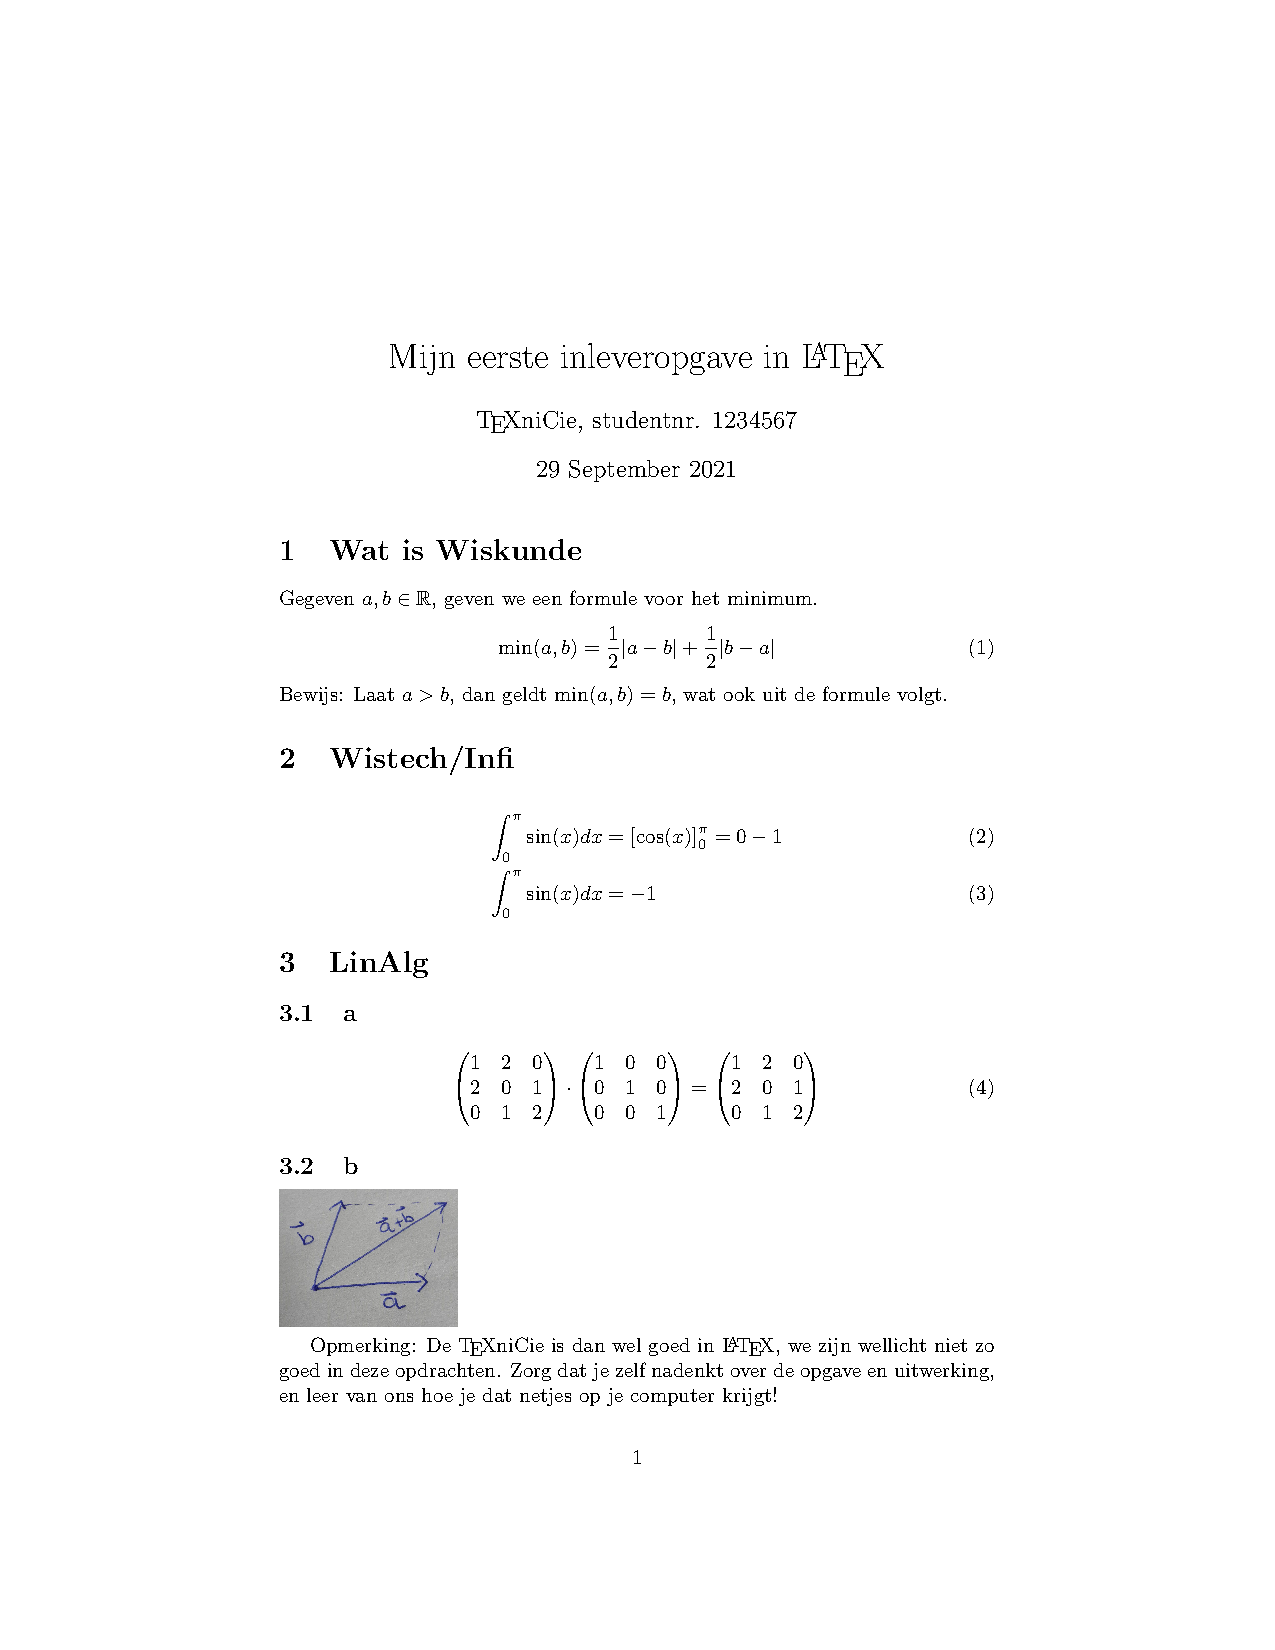
\includegraphics[width=0.4\textwidth]{assets/voorbeeldweek1.pdf}}
		& \fbox{\includegraphics[width=0.4\textwidth,page=2]{assets/voorbeeldweek2.pdf}}
	\end{tabular}
\end{frame}

\begin{frame}
	\frametitle{Wat we voor mogelijkheden zien:}
	\begin{itemize}
		\item Een header, inclusief links en rechts uitlijning
		\item Minder witruimte links en rechts op de pagina
		\item Lijsten in deel 1
		\item Plaatje met onderschrift
		\item Een footer met uitlijning en pagina zoveel van totaal
		\item (Misschien is je in de andere pagina's van het voorbeeld al meer opgevallen)
		\item Er is veel meer mogelijk, afhankelijk van je smaak en hoeveel werk je erin wil steken...
	\end{itemize}
\end{frame}

\importslide{text}{text-quotes.tex}


\importslide{document}{document-parts.tex}

\importslide{document}{document-margins.tex}

\begin{frame}
	\frametitle{Uitlijning en pagina-layout}
	Voor de paginamarges: \hll|\\usepackage\{geometry\}|

	Optioneel kan je echt alle dimensies van je document meegeven:
	\begin{figure}
			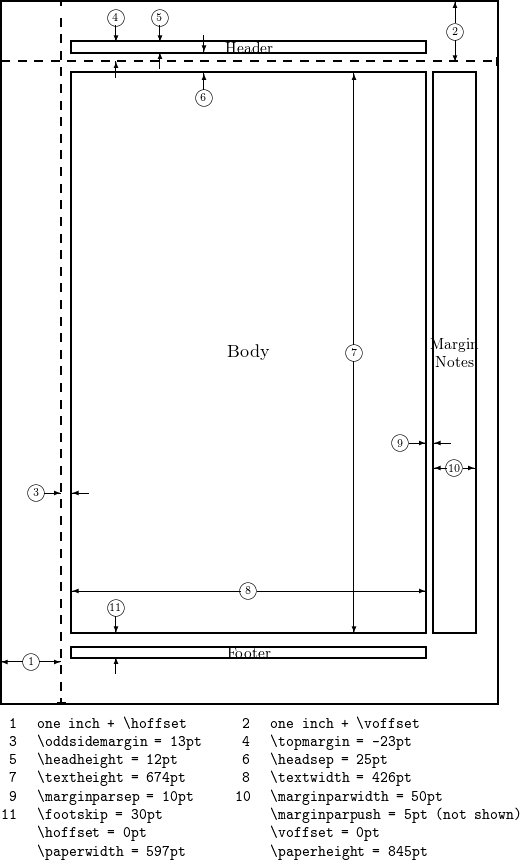
\includegraphics[height=0.9\textheight]{assets/Layout-dimensions.png}
			%\caption{Zoals je kan zien in dit plaatje op de site van Overleaf.}
	\end{figure}
\end{frame}

\importslide{document}{document-fancyhdr.tex}

\begin{saveblock}{fancyhdr}
    \begin{highlightblock}
        \usepackage{fancyhdr}
        \pagestyle{fancy}
        \fancyhf{}
        \rhead{Hier wat je rechts in je header uitgelijnd wil}
        \lhead{Hier wat je links in je header uitgelijnd wil}
        \rfoot{Hier wat je rechts in je footer uitgelijnd wil}
        \lfoot{Hier wat je links in je footer uitgelijnd wil}
    \end{highlightblock}
\end{saveblock}

\begin{frame}
	\frametitle{Headers en footers}
	Wellicht wil je op elke pagina van je inleveropgave iets neerzetten, zoals
	in het voorbeeld. De titelpagina heeft standaard een andere opmaak, zonder
	header en footer! Wat het wordt definieer je in de preamble:

    \useblock{fancyhdr}
\end{frame}

%\importslide{document}{document-sections.tex}

\importslide{document}{document-toc.tex}

\importslide{document}{document-secnumdepth.tex}

\importslide{document}{document-section_star.tex}

\importslide{document}{document-hyperref.tex}


\begin{frame}
	\frametitle{Andere handige layout codes}
	Voor het horizontaal opvullen/leeglaten van je (tekst)regel, minus wat je
	nog aan de rechterkant wil zetten kan je \hll|\\hfill|
	gebruiken:

	Links \hfill Rechts
	
	Voor het verticaal opvullen/leeglaten van je pagina, \vfill minus wat je nog
	onderaan wil zetten gebruik je \hll|\\vfill|.
\end{frame}

\begin{saveblock}{fancyhdr}
    \begin{highlightblock}
        \usepackage{fancyhdr,lastpage}
        \pagestyle{fancy}
        \fancyhf{}
        \rhead{Hier wat je rechts in je header uitgelijnd wil}
        \lhead{Hier wat je links in je header uitgelijnd wil}
        \rfoot{Pagina \thepage{} van \pageref{LastPage}}
    \end{highlightblock}
\end{saveblock}

\begin{frame}
	\frametitle{Oefening: maak de layout van voorbeeld van deze week}
	Probeer de opmaakelementen (dus niet de inhoudsopgave, deel 1, 2.1,  2.2 en de wiskunde van deel 3) na te maken in een nieuw document.
    
    \useblock{fancyhdr}
    
	Klaar? Bekijk de extra oefeningen van vorige week over tekstkleuren en
	groottes op
	\href{https://vkuhlmann.com/latex/exercises/2021-09-Cursus/week1}{\nolinkurl{vkuhlmann.com/latex/exercises/2021-09-Cursus/week1}}\\
	Weer klaar? Probeer de wiskunde van deel 3 toe te voegen.
    % (zoek symbolen op in de presentatie van vorige week of teken ze in
	% \url{detexify.kirelabs.org/}).
	
\end{frame}

\section{Figuren en tabellen}
% \begin{frame}
% 	\frametitle{Figuren}
% 	\begin{block}{code opzet}
% 		\texttt{\textbackslash begin\{figure\}[Plaatsbepaler]\\
% 			\textbackslash centering\\
% 			\textbackslash includegraphics[optionals]\{plaatje.png\}\\
% 			\textbackslash caption\{Onderschrift\}
% 			\textbackslash label\{fig:plaatje\}
% 		\textbackslash end\{figure\}}
% 	\end{block}
% 	\begin{block}{output}
% 	{\begin{figure}
% 	\centering
% 	%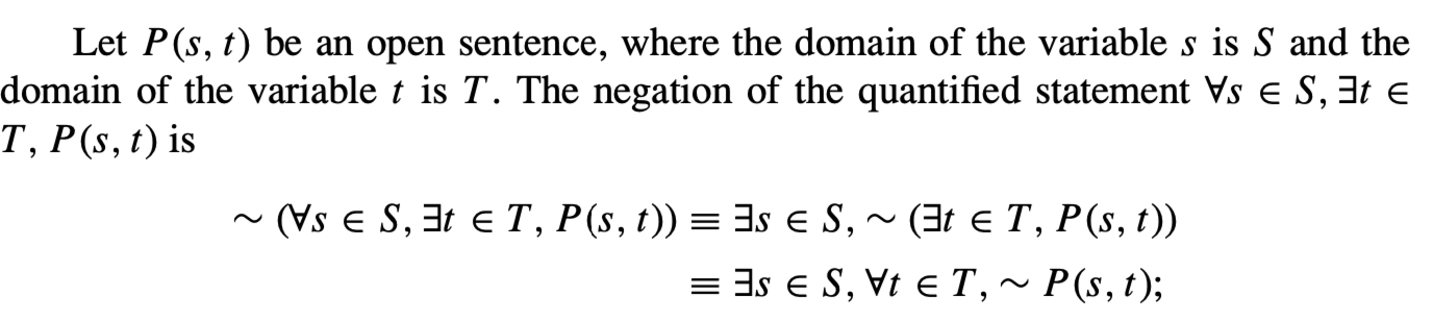
\includegraphics{plaatje.png}
%     \includegraphics[height=2cm]{example-image-a}
% 	\caption{Onderschrift}
% 	\label{fig:plaatje}
% 	\end{figure}}
% 	\end{block}
% \end{frame}
% \begin{frame}{Meerdere plaatjes in \'e\'en figuur omgeving}
% 	\texttt{\textbackslash begin\{figure\}\\
% 		\quad	\textbackslash begin\{subfigure\}[plaatsing]\{Breedte\}\\
% 			\qquad	\textbackslash centering\\
% 			\qquad	\textbackslash includegraphics...\\
% 			\qquad	\textbackslash caption\{onderschrift subfig a\}\\
% 			\qquad	\textbackslash label\{fig:subfiga\}\\
% 		\quad	\textbackslash end\{subfigure\}\\
% 		\quad	... code herhalen voor meer subfiguren ...\\
% 		\quad	\textbackslash caption\{onderschrift voor alle plaatjes bijelkaar\}\\
% 		\quad	\textbackslash label\{fig:subfigsabcde\}\\
% 		\textbackslash end\{figure\}
% 	}
% \end{frame}

\importslide{images}{includegraphics-asparagraph.tex}
\importslide{images}{includegraphics-center.tex}
\importslide{images}{includegraphics-figure.tex}

% \importslide{images}{figure-placement.tex}

\importslide{images}{figure-dimensions.tex}

\importslide{images}{subfigure.tex}

\importslide{images}{figure-placement.tex}

\begin{frame}[allowframebreaks]{De plaatsbepaler}
	% 	De plaatsbepaler is een argument [in deze recht haken dus] dat aangeeft waar je precies het figuur/de tabel hebben wilt. Deze precies is niet zo precies als je bij Word kan aangeven, waarschijnlijk krijg je er ooit ruzie mee dus we gaan ook wat oplossingen na.
	
	% \framebreak
	% Je kunt gebruik maken van de volgende plaatsbepalers:
	
	% \begin{table}
	% 	\center
	% 	\begin{tabular}{lll}
	% 		h &	here    & Plaats het figuur \alert{ONGEVEER} hier in de tekst. \\
	% 		t & top     & Plaats het figuur bovenaan de bladzijde.\\
	% 		b & bottom  & Plaats het figuur onderaan de tekst. \\
	% 		p &	page    & Plaats het figuur op een speciale pagina voor figuren. \\
	% 		! &	        & Dit commando kun je achter \'e\'en van de bovenstaande  \\ 
	% 		&         & plakken en overreed de interne parameters voor het\\
	% 		&         & vinden van een goede positie.\\
	% 		H & HERE    & Plaats het figuur precies \alert{HIER} in het document.\\
	% 		&         & Dit lijkt veel op het h! commando.
	% 	\end{tabular}
	% \end{table}
	% \framebreak
	
	Het maakt niet uit in welke volgorde h, p, t, b of ! staan, \LaTeX{} gebruikt de volgende volgorde: 
	\begin{itemize}
		\item Eerst kijkt het of er een h tussen staat. Als er een h is opgegeven, probeert \LaTeX{} meteen het figuur te plaatsen.
		\item Als dat niet gelukt is en er staat een t, probeert het het plaatje bovenaan te plaatsen.
		\item Daarna probeert \LaTeX{} een b.
		\item Als het plaatje nog steeds niet past, stopt \LaTeX{} het plaatje in de wachtrij. Deze wordt geleegd, als er een nieuwe pagina wordt aangemaakt.
	\end{itemize}
	\framebreak
	
	Veel gebruikte oplossingen om het plaatje toch te krijgen waar jij wil:
	\begin{itemize}
		\item Maak het plaatje kleiner zodat er minder problemen zijn
		\item Verplaats de code voor een plaatje iets naar voren om het plaatje
		wel op de juiste plek te krijgen
		\item Eindig je pagina na de tekst waarna je het plaatje wil en gebruik
		\hll|\\clearpage| zolang de rest van de pagina groot
		genoeg is voor het plaatje komt het plaatje onderaan.
		\item Kies ervoor alleen te refereren naar plaatjes in je tekst en alle
		plaatjes op een aparte pagina te zetten.
	\end{itemize}
We gaan eerst wat oefenen, voor we overgaan op de referenties.
\end{frame}

\begin{saveblock}{tabel}
    \begin{highlightblock}
        \begin{table}
            \centering
            \begin{tabular}{||r|c|l||}% <-- layout
                Rij1 & $\mathbb{WISKUNDE}$ & tekst\\
                Nieuwe regel & met net zoveel & als kolommen in
                de hele tabel\\
                \hline
                Laatste & regel & tabel
            \end{tabular}
            \caption{Onderschrift}
            \label{tab: tabel}
        \end{table}
    \end{highlightblock}
\end{saveblock}

\begin{frame}
	\frametitle{Tabellen}
	% \begin{block}{code opzet}
	% 	\texttt{\textbackslash begin\{table\}[Plaatsbepaler]\\
	% 	\quad	\textbackslash centering\\
	% 	\quad	\textbackslash begin\{tabular\}\{LAYOUT\}\}\\
	% 	\qquad	Rij1 \& \$wiskunde\$ \& tekst \textbackslash \textbackslash\\
	% 	\qquad	Nieuwe regel \& met net zoveel \& als kolommen in\\
	% 	\qquad de hele tabel\textbackslash
	% 		\textbackslash\\
	% 	\qquad	\textbackslash hline\\
	% 	\qquad	Laatste \& regel \& tabel\\
	% 	\quad	\textbackslash end\{tabular\}\\
	% 	\quad	\textbackslash caption\{Onderschrift\}\\
	% 	\quad	\textbackslash label\{tab:tabel\}\\
	% 		\textbackslash end\{table\}}
	% \end{block}
    \useblock{tabel}
\end{frame}

\begin{frame}
	\frametitle{Tabellen}
	Layout voor elke rij:
	\begin{itemize}
		\item \hll|l,c,r| voor uitlijning van elementen, net zoveel letters als kolommen
		\item je kan verticale lijnen maken door $|$ te plaatsen tussen de letters (dubbele lijnen door $||$)
	\end{itemize}
%Kies bijvoorbeeld \texttt{||r|c|l||}, dan ziet de tabel er zo uit:
	\begin{block}{Met layout \hll,||r|c|l||,}
		{\begin{table}
				\centering
				\begin{tabular}{||r|c|l||}
					Rij1 & $\mathbb{WISKUNDE}$ & tekst\\
					Nieuwe regel & met net zoveel & als kolommen in de hele tabel\\
					\hline
					Laatste & regel & tabel
				\end{tabular}
				\caption{Onderschrift}
				\label{tab: tabel}
		\end{table}}
	\end{block}
\end{frame}

\begin{frame}
	\frametitle{Oefenen met figuren en tabellen}
	Vul in je eerder gemaakte document sectie twee in met een leuk plaatje (mag
	ook iets anders zijn) en de gegeven tabel. Schrijf eerst nog letterlijk de
	captions over, straks kan je die in de tabel vervangen door een referentie.

	Klaar?	Voeg aan het eind van sectie 2 een plaatje toe (bijvoorbeeld van je
	favoriete dier), die precies geplaatst wordt tussen de tabel en de titel van
	sectie 3. Kijk ook of het je lukt hem helemaal bovenaan of onderaan de
	pagina te krijgen.
\end{frame}

\importslide{internals}{internals-spaces_in_code.tex}
	
\section{Referenties}

\begin{saveblock}{refWrong}
	\begin{highlightblock}[gobble=8,linewidth=\textwidth,
		framexleftmargin=0.25em,xleftmargin=0.25em]
		Zie pinguin in Figuur 1.
		\begin{figure} % <-- Figuur 1
			... % Pinguin
		\end{figure}
	\end{highlightblock}
\end{saveblock}

\begin{saveblock}{refWrong2}
	\begin{highlightblock}[gobble=8,linewidth=\textwidth,
		framexleftmargin=0.25em,xleftmargin=0.25em]
		\begin{figure} % <-- Figuur 1
			... % Man in tuxedo-pak
		\end{figure}
		Zie pinguin in Figuur 1.
		\begin{figure} % <-- Figuur 2
			... % Pinguin
		\end{figure}
	\end{highlightblock}
\end{saveblock}

\begin{frame}
	\frametitle{Referenties}

	\unless\ifishandout
	\only<1>{\useblock{refWrong}}
	\fi

	\only<2->{\useblock{refWrong2}}
\end{frame}

\begin{saveblock}{refCorrect}
	\begin{highlightblock}[gobble=8,linewidth=\textwidth,
		framexleftmargin=0.25em,xleftmargin=0.25em]
		\begin{figure} % <-- Figuur 1
			... % Man in tuxedo-pak
		\end{figure}
		Zie pinguin in Figuur \ref{fig:pinguin}.
		\begin{figure} % <-- Figuur 2
			... % Pinguin
			\caption{...}\label{fig:pinguin}
		\end{figure}
	\end{highlightblock}
\end{saveblock}

\begin{frame}
	\frametitle{Referenties}

	\useblock{refCorrect}
\end{frame}

\begin{frame}[allowframebreaks]
	\frametitle{Verwijzen}
	Stel je wil een extra plaatje op de voorpagina, dan wordt figuur 1 (in
	sectie 2) hernoemt naar figuur 2, het is immers nu het tweede figuur wat we
	plaatsen, maar nu staat er in het onderschrift van de tabel nog figuur 1!
	
	\LaTeX{} kan automatisch refereren naar het juiste nummer, zonder dat jij je
	zorgen hoeft te maken welk nummer die precies heeft gekregen. Sterker nog,
	dat kan ook met de \hll|align| en \hll|equation| omgevingen als je
	naar formules wil refereren. Handig als je een paar regels later een vorige
	formule wil gebruiken. Je kan ook naar secties en subsecties verwijzen.
	
	\framebreak
	
	Om te kunnen verwijzen moet je dingen een naampje geven. Dit doe je door het
	commando \alert{\hll|\\label\{fig:tekening\}|}. De conventie
	is om de eerste twee of drie letters te verwijzen naar wat voor soort iets
	het is, daarna een : om vervolgens een korte tekst te geven als omschrijving
	voor jezelf
	
	\begin{table}
		\centering
		\small\begin{tabular}{c|l}
			eq:&	equation \\ 
			fig:&	figure \\
			tab:&	table \\
			chap: &	chapter \\
			sec:&	section \\
			subsec:&	subsection \\
			itm:&	enumerated list item \\
			app:&	appendix subsection
		\end{tabular}
	\end{table}

	\framebreak
	Vervolgens refereer je terug aan je label door een commando. Er zijn verschillende gevallen:
	\begin{description}
		\item[handmatig:]
        Je kan zelf schrijven: \hll|Zie Figuur \\ref\{fig:tekening\}|.
		\item[automatisch] Het commando \hll|\\autoref\{fig:tekening\}| geeft als output
        \textit{Figuur 4}. 
		\item[pagina]  Het commando \hll|\\pageref| verwijst naar de pagina
		waarop iets is geplaatst (of begint als het langer is dan een pagina).
		\item[formule] gebruik \hll|Vergelijking \\eqref\{eq:vergelijking\}| \textit{voor Vergelijking (3)}.
	\end{description}
\end{frame}
	
\begin{frame}
	\frametitle{Taal}
	Pas hierbij op dat je de juiste taal gebruikt in \LaTeX, dat is het Babel
	package. Standaard staat die in het Engels en zullen je figuren dus
	\textit{Figure 4} heten en autorefereren naar \textit{Figuur 4}. Zet in je
	preamble \hll|\\usepackage[dutch]\{babel\}| om dit te
	veranderen naar Nederlandse namen.
\end{frame}	

\begin{frame}{Inhoudsopgave}
	Een inhoudsopgave is nog gemakkelijker dan \hll|\\maketitle|, waar je nog de
	titel, auteur en datum op moet geven. \LaTeX{} houdt namelijk automatisch je
	secties bij. Je print de inhoudsopgave met \hll|\\tableofcontents|. Dit
	gebeurt wel alleen bij secties die een nummer hebben. Iets wat niet
	automatisch in de inhoudsopgave komt handmatig toevoegen kan door
    \hll|\\addcontentsline\{toc\}\{section\}\{Naam\}|
	%\texttt{\textbackslash addto contentsline\{toc\}\{section\}\{Naam\}},
    waar \hll|toc| staat voor Table Of Contents, \hll|section| voor welk soort
	element en de laatste entry de naam is die verschijnt in de inhoudsopgave.
\end{frame}

\begin{frame}{oefenen}
	Vul je document aan met de referenties en inhoudsopgave. Probeer
	verschillende manieren en plekken om labels te plaatsen. Let vooral op de
	plaatsing van \hll|\\caption| en \hll|\\label| bij je plaatje!

	Klaar? Neem een koekje!
\end{frame}

\section{Lijsten}

\importslide{text}{text-lists.tex}

\begin{frame}{Itemize, enumerate}
	\begin{itemize}
		\item de itemize-omgeving geeft dit als output.
		\item gebruik code: \hll|\\begin\{itemize\}| \dots \hll|\\end\{itemize\}|
		\item tussendoor gebruik je bij elk deel van de tekst \hll|\\item|
		\item \hll|\\item| Het volgende punt wordt dus zo
		\item Het volgende punt wordt dus zo
	\end{itemize}
In plaats van itemize kan je ook \hll{enumerate} gebruiken voor getallen. Je kan
op elk moment een item laten nummeren met $n$ door voor het nieuwe item in de
code het commando \hll|\\setcounter\{enumi\}\{$n-1$\}| zetten
(volgende week meer over die counters).
\end{frame}

\begin{frame}{Description}
	Je kan ook een lijst maken die je een woord meegeeft ipv dat er een getal of
	punt staat, dat is de \hll|description| omgeving. Het woord geef je op de
	volgende manier mee:\\
	\hll|\\item[omschrijving]|.
\end{frame}

\begin{frame}{oefenen}
	Vul sectie 1 in je document op zoals in het voorbeelddocument van deze week.
\end{frame}

\begin{saveblock}{stelling}
    \begin{highlightblock}
        \begin{stelling}[Mijn eerste stelling]
            Laat $ a > b $, dan $ a - b > 0 $.
            \begin{proof}
                Haal $ b $ af van beide ...
                daarmee ...
            \end{proof}
        \end{stelling}
    \end{highlightblock}
\end{saveblock}

\section{Stellingen en bewijzen}
\begin{frame}[allowframebreaks]{Stellingen en bewijzen}
	Voor de wiskundestudenten is er ook een speciale omgeving zodat stellingen en bewijzen er netjes uitzien.
	Dit is de theorem omgeving uit het package \hll|amsmath|.
	In je preamble kan je aangeven wat voor soort omgevingen je wil maken.
    \hll|\\newtheorem\{stelling\}\{Stelling\}|
	
	\framebreak
	Op deze manier kan je bijvoorbeeld netjes een Stelling maken:
	% \begin{block}{code}
	% 	\texttt{\textbackslash begin\{stelling\}[Mijn eerste stelling]\\
	% 		Laat \$a>b\$, dan \$a-b>0\$.\\
	% 		\textbackslash end\{stelling\}\\
	% 		\textbackslash begin\{proof\}\\
	% 			Haal \$b\$ af van beide kanten van het ongelijkheidsteken, dit verandert niet de richting van het ongelijkheidsteken.\\
	% 		\textbackslash end\{proof\}}
	% \end{block}
    \useblock{stelling}
\end{frame}

\begin{frame}{Oefenen}
	Voeg de stelling van de vorige slide toe aan een vierde pagina van je document. Zorg dat, waar dat nog niet zo is, de rest van je document vergelijkbaar is met het voorbeelddocument van week 2.
	\vfill
	NB: zowel deze slides als dat voorbeeld staan op onze site: \url{www.a-eskwadraat.nl/latex}
\end{frame}


\section{\texorpdfstring{}{Misc}}

\importslide{misc}{misc-contact.tex}

% \begin{frame}
% 	\frametitle{Volgende keer -- Week 3 (di 12 okt): Verdiepend}

% 	\begin{multicols}{2}
% 		\begin{itemize}
% 			\item AA
% 			\item BB
% 			\item Meer
% 		\end{itemize}\par
% 		\vfill
% 		\leavevmode
% 	\end{multicols}

% 	(Voorbeeld van wat je bereikt is te vinden op)
% 	\begin{center}
% 		\href{https://a-eskwadraat.nl/latex}{\ul{\texttt{a-eskwadraat.nl/latex}}}
% 	\end{center}

% 	\medskip
% 	Inschrijven nog mogelijk!
% \end{frame}

% \begin{frame}
% 	Oefeningen!
% \end{frame}

% \ifishandout
% 	\importslide{misc}{misc-license.tex}
% \fi
	
\end{document}
